\documentclass{article}
\usepackage{tikz}

\begin{document}

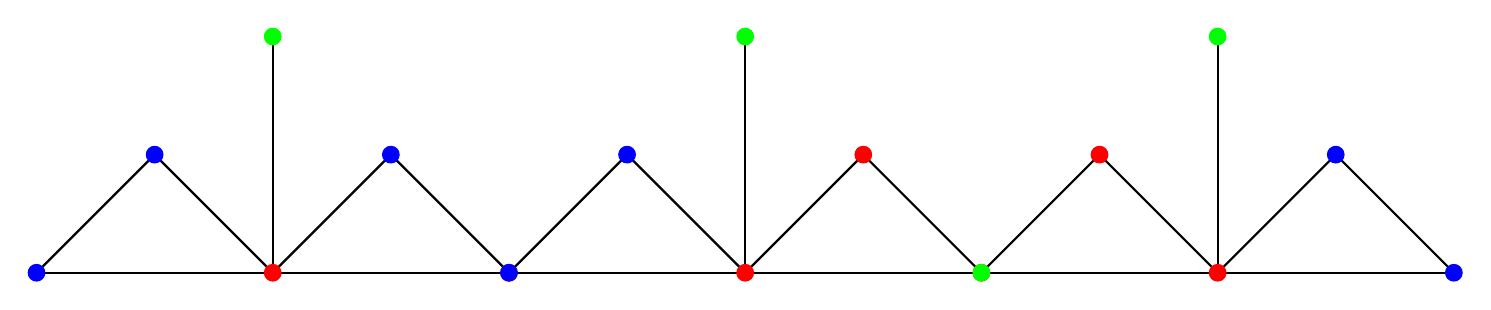
\begin{tikzpicture}[scale=1.5]
    % Define colors
    \definecolor{red}{RGB}{255,0,0}
    \definecolor{blue}{RGB}{0,0,255}
    \definecolor{green}{RGB}{0,255,0}

    % Graph 1
    \draw[thick] (0,0) -- (1,1);
    \draw[thick] (0,0) -- (-1,1);
    \draw[thick] (0,0) -- (0,2);
    \draw[thick] (1,1) -- (2,0);
    \draw[thick] (-1,1) -- (-2,0);
    \draw[thick] (2,0) -- (-2,0);

    \filldraw[red] (0,0) circle (2pt);
    \filldraw[blue] (1,1) circle (2pt);
    \filldraw[blue] (-1,1) circle (2pt);
    \filldraw[green] (0,2) circle (2pt);
    \filldraw[red] (2,0) circle (2pt);
    \filldraw[blue] (-2,0) circle (2pt);

    % Graph 2
    \begin{scope}[xshift=4cm]
        \draw[thick] (0,0) -- (1,1);
        \draw[thick] (0,0) -- (-1,1);
        \draw[thick] (0,0) -- (0,2);
        \draw[thick] (1,1) -- (2,0);
        \draw[thick] (-1,1) -- (-2,0);
        \draw[thick] (2,0) -- (-2,0);

        \filldraw[red] (0,0) circle (2pt);
        \filldraw[red] (1,1) circle (2pt);
        \filldraw[blue] (-1,1) circle (2pt);
        \filldraw[green] (0,2) circle (2pt);
        \filldraw[red] (2,0) circle (2pt);
        \filldraw[blue] (-2,0) circle (2pt);
    \end{scope}

    % Graph 3
    \begin{scope}[xshift=8cm]
        \draw[thick] (0,0) -- (1,1);
        \draw[thick] (0,0) -- (-1,1);
        \draw[thick] (0,0) -- (0,2);
        \draw[thick] (1,1) -- (2,0);
        \draw[thick] (-1,1) -- (-2,0);
        \draw[thick] (2,0) -- (-2,0);

        \filldraw[red] (0,0) circle (2pt);
        \filldraw[blue] (1,1) circle (2pt);
        \filldraw[red] (-1,1) circle (2pt);
        \filldraw[green] (0,2) circle (2pt);
        \filldraw[blue] (2,0) circle (2pt);
        \filldraw[green] (-2,0) circle (2pt);
    \end{scope}
\end{tikzpicture}

\caption{Maximal case (up to isomorphism) where \( u \) and \( v \) do not have a common neighbor and \( G \) has a triangle. Even this maximal case is \( 3 \)-colorable.}

\end{document}